

\tikzset{every picture/.style={line width=0.75pt}} %set default line width to 0.75pt        

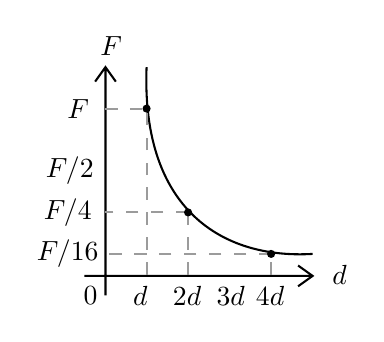
\begin{tikzpicture}[x=0.75pt,y=0.75pt,yscale=-1,xscale=1]
%uncomment if require: \path (0,300); %set diagram left start at 0, and has height of 300

%Shape: Axis 2D [id:dp41309470594896225] 
\draw  (50,170.6) -- (160,170.6)(60.2,70) -- (60.2,180) (153,165.6) -- (160,170.6) -- (153,175.6) (55.2,77) -- (60.2,70) -- (65.2,77)  ;
%Curve Lines [id:da3846708650107995] 
\draw    (80,70) .. controls (77.4,138.6) and (116.6,162.6) .. (160,160) ;


%Straight Lines [id:da08214510272188957] 
\draw [color={rgb, 255:red, 155; green, 155; blue, 155 }  ,draw opacity=1 ] [dash pattern={on 4.5pt off 4.5pt}]  (60,90) -- (80,90) ;


%Straight Lines [id:da8439893003808838] 
\draw [color={rgb, 255:red, 155; green, 155; blue, 155 }  ,draw opacity=1 ] [dash pattern={on 4.5pt off 4.5pt}]  (80,170) -- (80,90) ;


%Straight Lines [id:da05529270042861656] 
\draw [color={rgb, 255:red, 155; green, 155; blue, 155 }  ,draw opacity=1 ] [dash pattern={on 4.5pt off 4.5pt}]  (100,170) -- (100,140) ;


%Straight Lines [id:da6412447500082621] 
\draw [color={rgb, 255:red, 155; green, 155; blue, 155 }  ,draw opacity=1 ] [dash pattern={on 4.5pt off 4.5pt}]  (100,140) -- (60,140) ;


%Straight Lines [id:da6265249084506017] 
\draw [color={rgb, 255:red, 155; green, 155; blue, 155 }  ,draw opacity=1 ] [dash pattern={on 4.5pt off 4.5pt}]  (140,170) -- (140,160) ;


%Straight Lines [id:da16502512531713776] 
\draw [color={rgb, 255:red, 155; green, 155; blue, 155 }  ,draw opacity=1 ] [dash pattern={on 4.5pt off 4.5pt}]  (140,160) -- (60,160) ;


%Shape: Circle [id:dp7563779977577021] 
\draw  [fill={rgb, 255:red, 0; green, 0; blue, 0 }  ,fill opacity=1 ] (138.58,160) .. controls (138.58,159.22) and (139.22,158.58) .. (140,158.58) .. controls (140.78,158.58) and (141.42,159.22) .. (141.42,160) .. controls (141.42,160.78) and (140.78,161.42) .. (140,161.42) .. controls (139.22,161.42) and (138.58,160.78) .. (138.58,160) -- cycle ;
%Shape: Circle [id:dp6638002256320048] 
\draw  [fill={rgb, 255:red, 0; green, 0; blue, 0 }  ,fill opacity=1 ] (98.58,140) .. controls (98.58,139.22) and (99.22,138.58) .. (100,138.58) .. controls (100.78,138.58) and (101.42,139.22) .. (101.42,140) .. controls (101.42,140.78) and (100.78,141.42) .. (100,141.42) .. controls (99.22,141.42) and (98.58,140.78) .. (98.58,140) -- cycle ;
%Shape: Circle [id:dp27247390199729726] 
\draw  [fill={rgb, 255:red, 0; green, 0; blue, 0 }  ,fill opacity=1 ] (78.58,90) .. controls (78.58,89.22) and (79.22,88.58) .. (80,88.58) .. controls (80.78,88.58) and (81.42,89.22) .. (81.42,90) .. controls (81.42,90.78) and (80.78,91.42) .. (80,91.42) .. controls (79.22,91.42) and (78.58,90.78) .. (78.58,90) -- cycle ;

% Text Node
\draw (63,60) node   {$F$};
% Text Node
\draw (173,170) node   {$d$};
% Text Node
\draw (47,90) node   {$F$};
% Text Node
\draw (43,120) node   {$F/2$};
% Text Node
\draw (42,140) node   {$F/4$};
% Text Node
\draw (42,160) node   {$F/16$};
% Text Node
\draw (53,180) node   {$0$};
% Text Node
\draw (77,180) node   {$d$};
% Text Node
\draw (99.5,180) node   {$2d$};
% Text Node
\draw (120.5,180) node   {$3d$};
% Text Node
\draw (139.5,180) node   {$4d$};


\end{tikzpicture}